\section{Background}
\label{sec:background}

\subsection{Coherent Combining in Distributed MIMO}
\label{sec:simo}

Wireless radios leverage multiple antennas (MIMO or multiple-input multiple-output) to improve throughput. This paper considers coherent combining where transmissions from a single-antenna transmitter (e.g. an LP-WAN client) are heard by multiple receiver antennas (e.g. LP-WAN gateways). These gateways can then coherently combine the received signals to improve signal decodability. 

% \subsection{Single-Input Multiple-Output}
% \label{sec:simo}

% Wireless devices have transitioned to using multiple antennas to leverage
% gains from on both client devices and access points. These are known as
% multiple-input multiple-output (MIMO) systems and their design involves using
% simultaneous transmissions and receptions from different antennas to obtain
% higher throughput, than what would be possible using any given pair of
% antennas on a transmitter and receiver. MIMO systems can provide higher
% throughput and resilience due to their ability to coherently combine signals
% both at the transmitter (known as \textit{beamforming}) and the receiver
% (known as \textit{diversity}). In traditional MIMO system such as those found
% in 802.11n, the various receiver antennas are a part of the same device which
% makes it easier to synchronize and combine the different receiver channels.
% However, distributed MIMO systems allow the receivers to be completely
% independent devices and still be able to coherently combine the received
% signals. Single-input multiple-output (SIMO) as shown in \figref{simo} is a
% subset of distributed MIMO systems where the transmitter only uses a single
% antenna. The LoRaWAN scenario we explore in this paper is based on SIMO
% systems.


Mathematically, let the transmitted signal be $x$ and each of the gateways receive a signal $y_i$ through wireless channel $h_i$, introducing an independent noise $n_i$ at the receivers. For a narrow-band system (as is LoRaWAN and most LP-WAN technologies), we can write the received signal as: $y_i = h_i x_i + n_i $. 

% Let the transmitted signal be $x$ and each of the gateways receive a signal
% $y_i$ through an AWGN channel that introduces independent noise $n_i$ at the
% receivers. A signal can be successfully decoded if its SNR is above a 
% threshold determined by the radio physical layer and the receiver hardware. 
% LoRa modulated signals are narrowband (up to 500 $kHz$) and
% their symbol periods are large ($> 256~\mu s$) to remain
% unaffected by inter-symbol interference. We thus have the following simplified
% channel model.


The receivers can now coherently combine their received signals by using the known wireless channels $h_i$:
\begin{align*}
y_{\text{combined}}
	= \sum_{i=1}^N h^*_i y_i
	= \sum_{i=1}^N \left| h_i \right|^2 x + \sum_{i=1}^N h^*_i n_i
\end{align*}

The first term is the combined signal while the second term is the combined
noise. However, while the signals add up coherently, the noise being
independent, adds up incoherently.  This results in an overall increase in the
combined signal-to-noise ratio (SNR) which allows us to jointly decode a packet that may otherwise not be decodable by any individual receiver.
\begin{align*}
SNR_{\text{combined}} %= \frac{\text{total signal power}}{\text{total noise power}} 
	= \frac{\left| \sum_{i=1}^N \left| h_i \right|^2 x \right|^2}{\sum_{i=1}^N \left| h^*_i n_i \right|^2} 
	\geq \frac{\left| \left| h_i \right|^2 x \right|^2}{\left| h^*_i n_i \right|^2} = SNR_i
\end{align*}

In practice, performing coherent combining as shown above makes two important assumptions: (1) the packets can be detected at individual receivers above some SNR threshold, and (2) receivers can share a common clock reference for time and frequency. This paper describes the challenges in implementing coherent combining in the low-power wide-area context where neither assumption holds. 

\begin{figure}[htb]
    \centering
    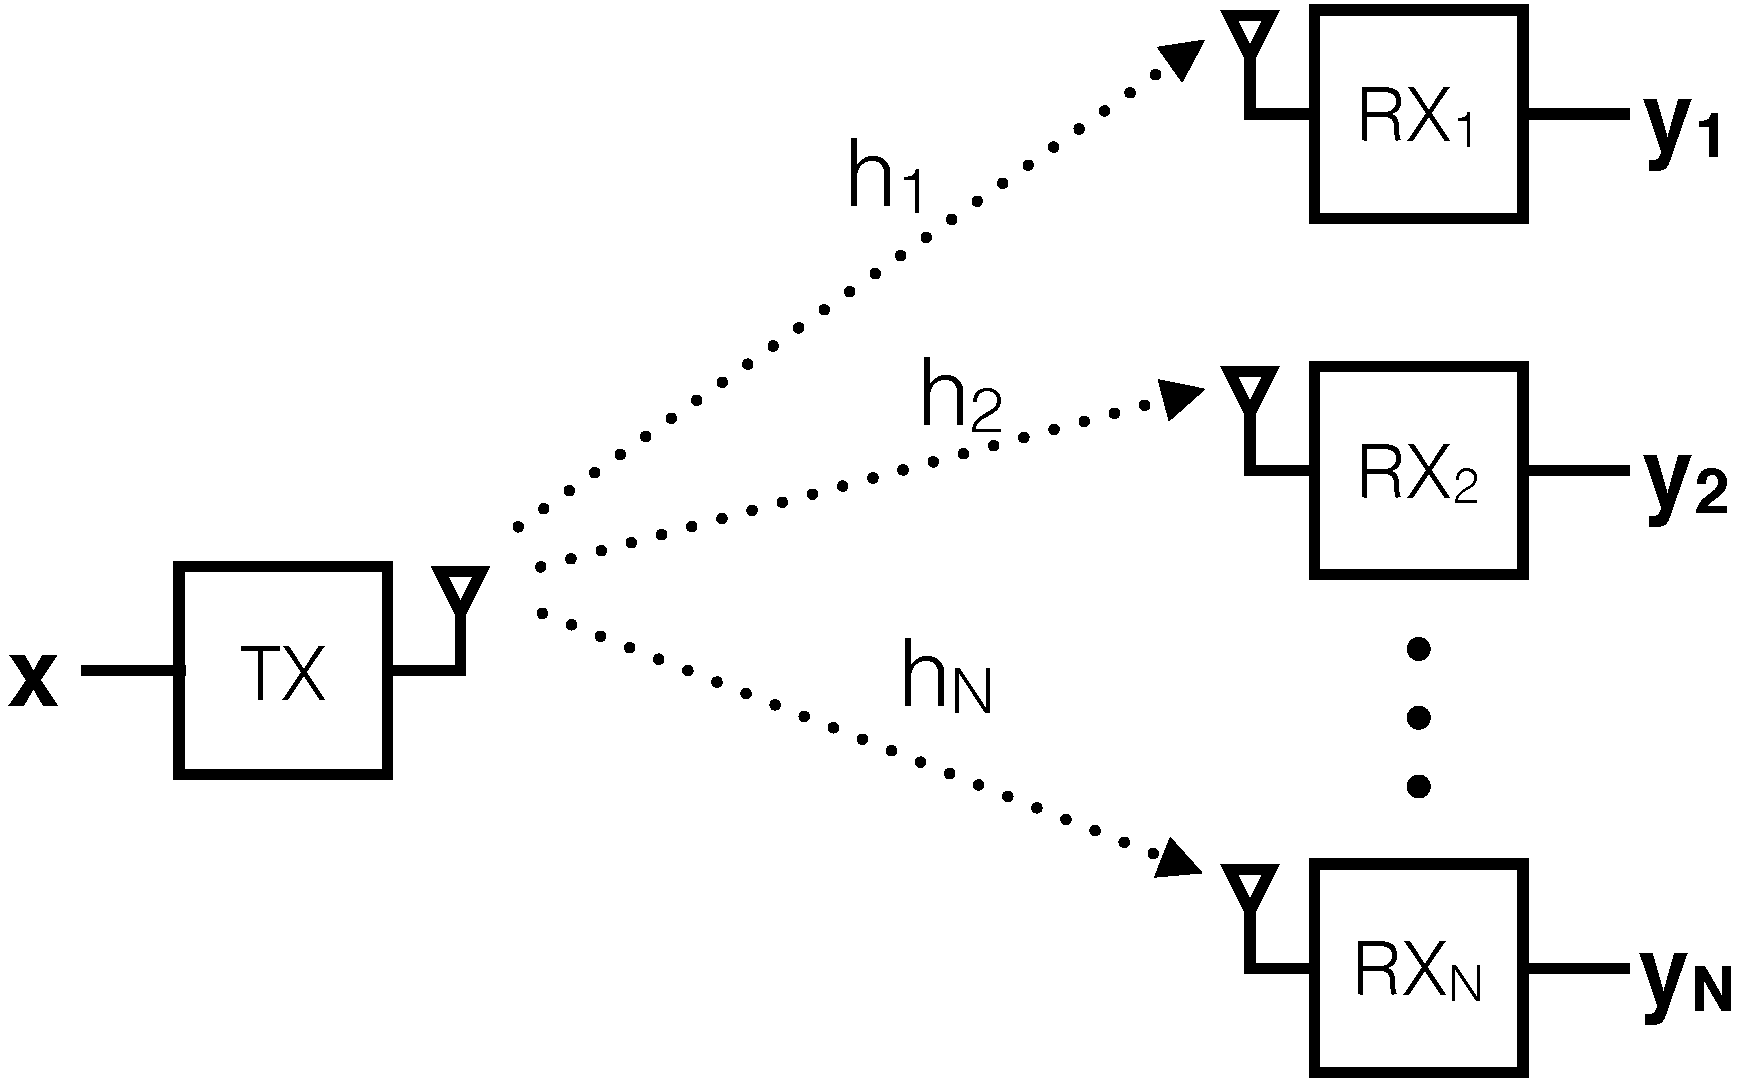
\includegraphics[height=1.25in]{figures/SIMO_cropped}
    %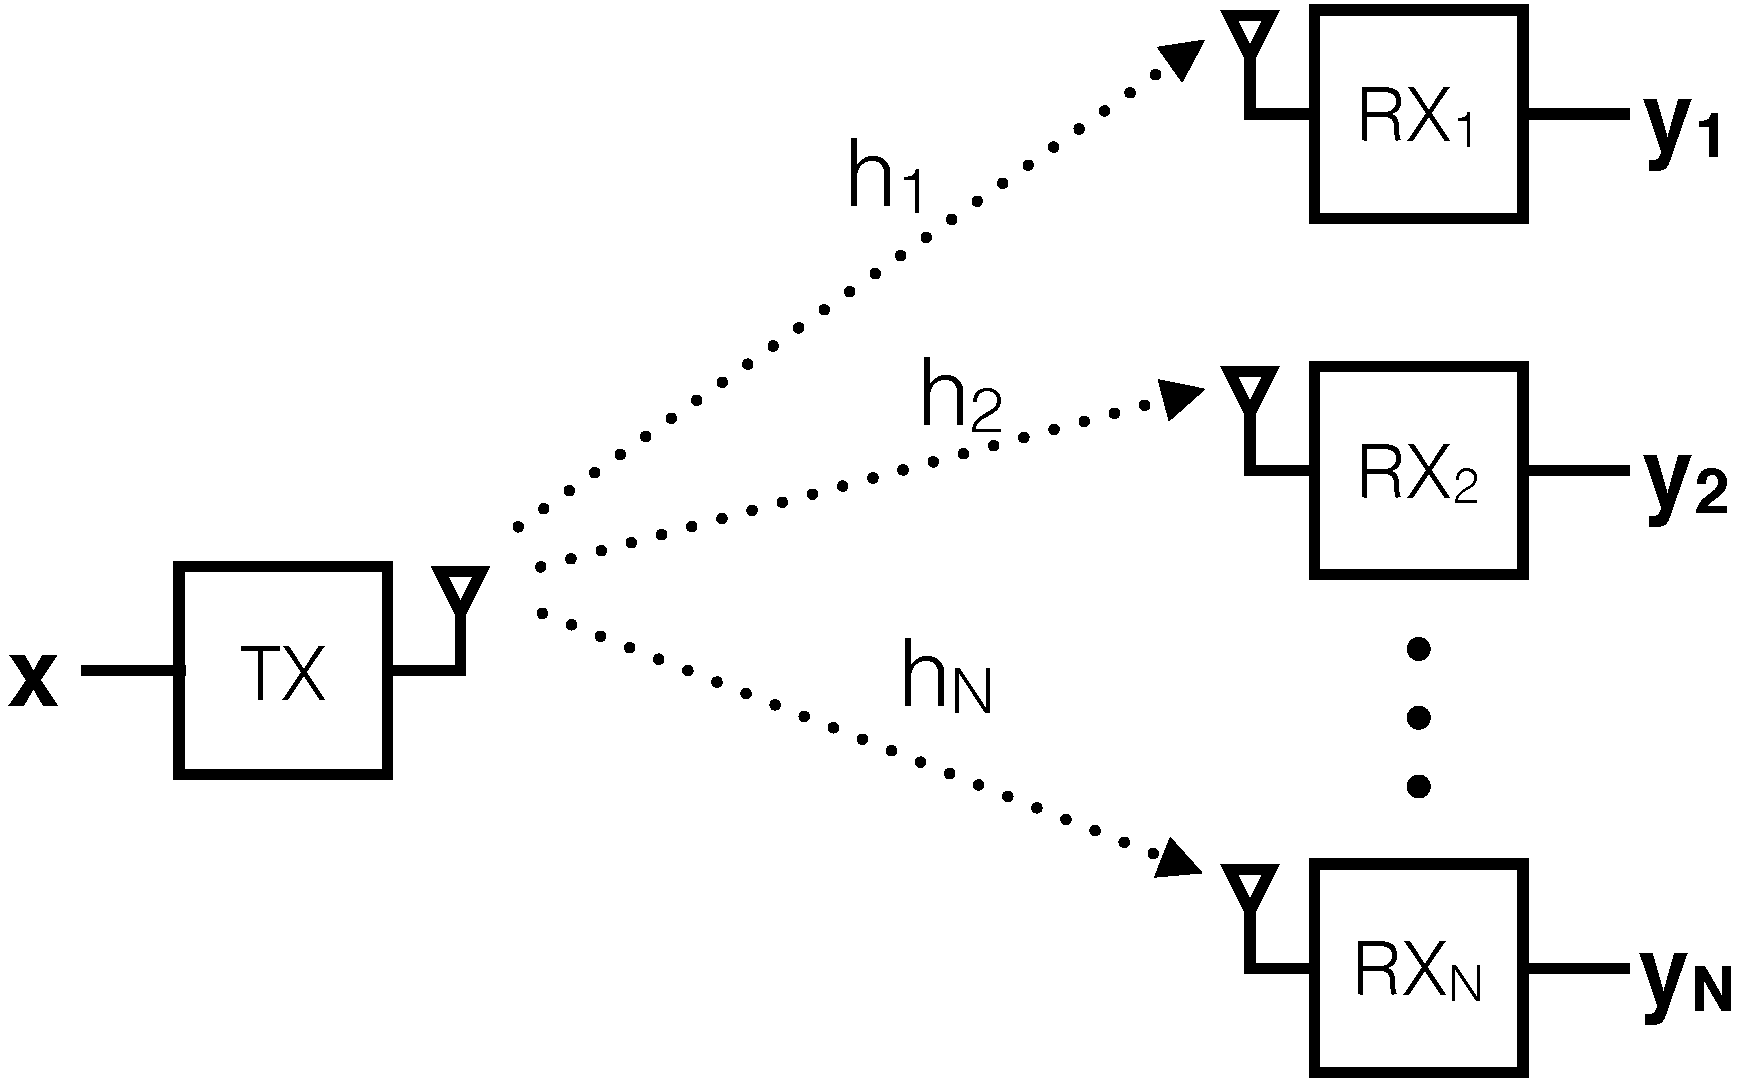
\includegraphics[width=0.35\textwidth, height=1in]{figures/SIMO_cropped}
    \caption{Coherent combining helps receives collaboratively improve signal-to-noise ratio}
    \label{fig:simo}
\end{figure}

\subsection{Primer on LoRaWAN PHY and MAC}
\label{sec:lora}

LoRaWAN is a popular LP-WAN technology that operates in the sub-GHz ISM band (900 MHz in the U.S.) and bandwidths of 125-500kHz. LoRaWAN clients can transmit at low-data rates (few kbps) to gateways up to 10 km away in free space and last up to 10-years on a coin-sized Li-Ion battery. Below, we detail a few key design decisions of LoRaWAN.\vspace*{0.02in}

\noindent \textbf{The PHY: } LoRa's physical layer is based on chirp-spread spectrum modulation i.e. using a chirp signal that continuously varies in frequency. This makes  it resilient to interference, multi-path fading and doppler effects. Every LoRaWAN packet begins with a preamble of sixteen repeated chirps, followed by data. Each data chirp encodes multiple data bits, with the number of  bits encoded per chirp called the \textit{spreading factor} (SF). For instance, at spreading factor of seven, each chirp encodes 7 bits with $2^7 = 128$ possible uniformly separated initial frequencies. A higher spreading factor, e.g. eight, encodes one more bit per chirp but also incurs double the transmission time, effectively halving the data rate.\footnote{More precisely, increasing spreading factor from $n$ to $n+1$ scales data rate by $(n+1)/2n$.} Increased spreading factors are used to simultaneously slow down transmissions and improve resilience to noise. LoRaWAN radios are therefore designed to transmit at the lowest possible spreading factor that current levels of noise support, in order to minimize transmission time and the resulting battery drain. This paper therefore strives to reduce spreading factor (improve data rate) for weak transmitters. 

% These
% characteristics enable successful reception of a transmission upto 27 dBm 
% below the  noise floor of the receiver. Transmissions occupy 125 to 500 kHz of bandwidth, which lets multiple independent frequency channels to co-exist in the sub-GHz ISM band (and allows additional features like frequency-hopping). Existing LoRa radios for client devices can transmit with up to 20 dBm power without additional power amplifiers. This modulation scheme enables low-power, long-range and high-efficiency operation but at the cost of long transmit time and low data rates.


% LoRa modulation, marketed by Semtech, is designed for long-range, unlicensed sub-GHz
% ISM band communication (900 MHz in the U.S., 868 MHz in Europe and similar bands elsewhere).
% LoRa's physical layer is based on chirp-spread spectrum modulation i.e. 
% using a chirp signal that continuously varies in frequency. This makes 
% it resilient to interference, multi-path fading and doppler effects. These
% characteristics enable successful reception of a transmission upto 27 dBm 
% below the  noise floor of the receiver. Transmissions occupy 125 to 500 kHz of bandwidth, which lets multiple independent frequency channels to co-exist in the sub-GHz ISM band (and allows additional features like frequency-hopping). Existing LoRa radios for client devices can transmit with up to 20 dBm power without additional power amplifiers. This modulation scheme enables low-power, long-range and high-efficiency operation but at the cost of long transmit time and low data rates.

% Similar to CDMA codes, LoRa modulation has a configurable parameter 
% called \textit{spreading factors}, defined as the ratio between the 
% symbol rate and the chip rate, that enables multiple simultaneous 
% transmission using the same frequencies. Every bit of information is mapped to multiple chips
% which are then modulated as up-chirps or down-chirps. As an example, at SF = 7, 128 chips are used for every symbol while 4096 chips are used for every SF = 12 symbol. Using a higher SF increases the SNR and consequently the sensitivity and range, but this also increases the transmission time of a message. Each level of the SF doubles the number of chips to be transmitted, thus decreasing the data-rate by half and increasing the energy consumption.

% Each bit of
% the message is embodied into multiple chips of information that are encoded as
% up-chirps or down-chirps (\figref{upchirp}). Furthermore, %The number of chips user per symbol is determined by the formula in equation~\eqref{SFequation}.
% For example, when using a \ac{SF} of 6 (SF6), 64 chips are used for every
% symbol, correspondingly 128 and 4096 are used for SF7 and SF12. The use of
% this modulation results in the capability of receiving signals with negative
% \ac{SNR} of up to 19.5 dB below the noise floor. In comparison, most \ac{FSK}
% systems need 8 to 10 dB above the noise floor in order to demodulate properly,
% resulting in more than 27 dB difference in the link budget between the two
% modulation systems, thus greatly increasing the range of a \ac{LoRa}
% system~\cite{SX1276,SX1301}.


% \subsubsection{Coding Rate (CR)}
% Coding Rate (CR) is the \ac{FEC} used by the LoRa modem that offers protection against bursts of interference.
% The sender adds redundancy in the messages by the use of \acp{ECC}.
% By default, \ac{LoRa} packet frames are encoded with the minimum CR of 4/5.
% A \ac{FEC} of 4/5 means that 4 useful bits are encoded into 5 transmission bits.
% As show in \tableref{FEC}, a higher CR offers more protection, but increases time on air.

% \subsubsection{Frame Structure}
% The LoRa frame structure is composed of four main
% fields {\color{blue} (point to LoRa spec or datasheet)}. It starts with the preamble that is programmable from 6 to 65535 symbols, to which the radio adds an additional 4.25 symbols. The preamble is followed by an optional frame header, which describes the length and FEC parameters of the payload, and indicates the presence of an optional CRC. The payload can contain 1 to 255 bytes and may be followed by a 16-bit optional CRC. The default preamble size of 16 produces a very characteristic signal which we exploit in Charm to enable local detection of very weak transmissions.

% \begin{figure}
%   \centering
%   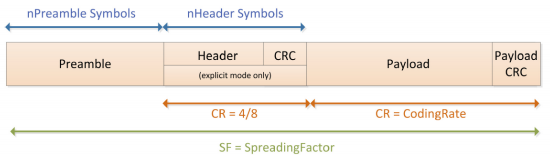
\includegraphics[width=\columnwidth]{figures/frame.png}
%   \caption{LoRa PHY Frame Structure (with permission~\cite{SX1276})}
%   \label{fig:frame}
% \end{figure}

% \subsubsection{LoRa Gateway}
% The only gateway \ac{LoRa} chip currently on the market is the SemTech SX1301.
% It has two radios fronends with four programmable reception channels each.
% Each of the channels has a fixed channel bandwidth of 125 kHz and their frequency can be individually configured to use any of the two radios.
% For each channel, it is able to detect preambles corresponding to all data rates (SF7 to SF12) at all times.
% However, the gateway cannot demodulate more than eight packets simultaneously, because the SX1301 architecture separates the preamble detection from the data demodulation process (i.e the SX1301 only has eight demodulation blocks).
% Theoretically, it is possible to demodulate up to six transmissions per channel, one for each \ac{SF}, but SemTech has restricted the number of demodulation blocks.
% Therefore, the SX1301 was primarily designed to detect the preambles within a channel.
% SemTech states that personalized customer circuit designs with more than eight demodulation blocks can be made on request.

% The SX1301 has an separate \ac{GFSK} reception channel with adjustable bandwidth and bitrate, that can demodulate any legacy \ac{FSK} OR \ac{GFSK} signal.
% It also include an additional channel that is intended to be used as a high speed back-haul link to other gateways or infrastructure.
% It uses a fixed 125khz, 250khz or 500khz bandwidth and \ac{SF}, similar to the SX1276 chips found in client devices~\cite{SX1301}.

% \subsubsection{Spectrum Regulation}
% In different part of the world, the allocated bandwidth, frequency and local
% regulations differ from each other. Even though LoRa operates using
% unregulated spectrum, the increase in dwell time (Air-Time) rises the
% probability of a collision in a contention based medium access. Thus, local
% regulations may enforce duty-cycle or dwell time restrictions for certain
% frequencies in order to implement fair use and avoid spectrum stagnation.

% The \ac{ETSI} has implemented such regulation on the European 868 MHz band that has 7 MHz of usable bandwidth.
% The regulations require the radio emitters to adopt duty-cycled transmission of 10\%, 1\% or 0.1\% depending on the sub-band.
% These transmissions also have a maximum transmit power as shown in table \tableref{DutyCycle}.
% In order to avoid duty-cycle limits, the transmitters need to implement two mechanisms: \ac{LBT} and \ac{AFA}.
% Both form a carrier sense mechanism that allow to sense the radio environment an only transmit on channels that are not yet occupied~\cite{ETSICompliance}.

% The \ac{FCC}, which is the regulatory body in the \ac{US}, has no frequency
% duty-cycle restrictions on the 915 MHz \ac{ISM} band that offers a total of 26
% MHz of bandwidth. Instead, they require each radio emitter to adopt a
% \ac{FHSS} scheme. Channel hopping should be employed in a pseudo-random nature
% across at least 25 or 50 channels in order to be able to transmit at a peak
% power output of +24 dBm (250 mW) and 30 dBm (1 W) respectively. Each
% transmission should not exceed a dwell time of 400 milliseconds within a
% period of 20 seconds~\cite{FCC15, FCCCompliance}. The maximum dwell time makes
% the lowest \ac{LoRa} data-rates (\ac{SF} 11 and 12) not usable, as
% transmitting the preamble alone already takes longer than 400 milliseconds.


\vspace*{0.02in}

\noindent \textbf{The MAC: }  LoRaWAN networks
are designed to be simple star-topologies that have client devices directly
communicating with a gateway that is connected to the internet over ethernet
or cellular links. Gateways are very simple and relatively inexpensive forwarders that send received packets to a cloud LoRaWAN server and can be commanded by the server to transmit data to clients at a specific time. Packet decoding, managing acknowledgements and
MAC parameters like data-rate and power-level are decided at a LoRaWAN
server. The LoRa community often refers to the system as having a
``MAC-in-the-Cloud'' design. LoRaWAN allows and encourages its users to deploy their own gateways. In this
paper, we refer to these as user-deployed gateways (UGW). These gateways are
completely unplanned and on low-bandwidth, unreliable internet connections
(compared to cellular base-stations which are extensively planned and have
dedicated optic fiber connections). The goal of this paper is to make individual unreliable user gateways more reliable by pooling together PHY-layer processing at the cloud.  


% \subsection{LoRaWAN}
% \label{sec:lorawan}

% The LoRa Wide-Area Networking (LoRaWAN) protocol works on top of the LoRa
% modulation layer to create an LP-WAN network capable of bi-directional data
% transfer. Its functionality is analogous to the Networking and transport
% layers (layers three and four) in the typical OSI design. LoRaWAN networks
% are designed to be simple star-topologies that have client devices directly
% communicating with a gateway that is connected to the internet over ethernet
% or cellular links. LoRaWAN defines three main device classes: bi-directional
% end-devices with downlink followed by uplink (Class A), bi-directional
% end-devices with transmission slots scheduled for downlink (Class B) and
% always-on bi-directional devices (Class C). Class A is primarily intended for
% sensors, Class B is intended for sensors with actuators while Class C is
% intended for powered devices that require low-latency. Gateways are very
% simple and relatively inexpensive forwarders that send received packets to a
% cloud LoRaWAN server and can be commanded by the server to transmit data to
% clients at a specific time. Packet decoding, managing acknowledgements and
% MAC parameters like data-rate and power-level are decided at a LoRaWAN
% server. The LoRa community often refers to the system as having a
% ``MAC-in-the-Cloud" design.

% LoRaWAN allows and encourages its users to deploy their own gateways. In this
% paper, we refer to these as user-deployed gateways (UGW). These UGWs are
% completely unplanned and on low-bandwidth, unreliable internet connections
% (compared to cellular base-stations which are extensively planned and have
% dedicated optic fiber connections). In pilot deployments, we've observed the
% same transmission being received by multiple gateways. In this paper, we
% leverage this observation combined with the diversity from unplanned UGW
% deployments to extend the coverage of higher data-rates in our network.
% Low-power devices which can now transmit at higher data rates thus end up
% saving energy to shorter transmit time.